\chapter{Why use typed Python\label{discussion}}  
% Or just discussion - the text here is very discussiony

\section{Why use Python}
Python's popularity can be attributed to several factors:

\begin{itemize}
    \item Python's design goals have led to a programming language that is simple to read, quick to write, and easy to learn. Effectively no popular statically typed languages have a similar design focus on developer experience.
    \item The ease of learning Python leads to it being a popular first programming language to learn, which leads it to have a large developer base.
    \item Useful packages are widely available. There is excellent support for various use cases, including scientific computing, machine learning, web development, desktop software development, and automation. 
% secret TODO: add more items
\end{itemize}

\section{Why type annotate Python}

Research on Python Type annotations focuses on how they are used, and their benefits and adoption patterns. It is rare to analyse why they are adopted.

In practice developers using type annotations are not aiming for completely typed Python programs. As can be seen from the amount of type errors present in most Python projects in the wild \cite{di_grazia_evolution_2022, rak-amnouykit_taleoftwo_2020,}, developers are utilizing the fact that a gradual type system enables gradually typing projects.

\begin{figure}[ht]
    \centering
    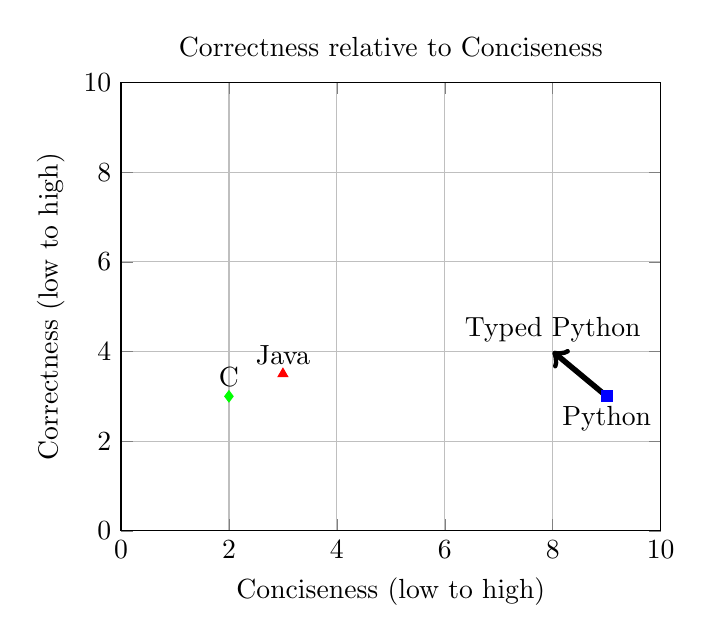
\begin{tikzpicture}
        \begin{axis}[
            xlabel={Conciseness (low to high)},
            ylabel={Correctness (low to high)},
            xmin=0, xmax=10,
            ymin=0, ymax=10,
            grid=major,
            legend pos=north west,
            title={Correctness relative to Conciseness}
        ]
        % Points for each language
        \addplot[only marks, mark=square*, color=blue] coordinates {(9, 3)}; % Python
        %\addplot[only marks, mark=square*, color=blue] coordinates {(8, 4)}; % typed Python
        \addplot[only marks, mark=triangle*, color=red] coordinates {(3, 3.5)}; % Java
        \addplot[only marks, mark=diamond*, color=green] coordinates {(2, 3)}; % C
        % \addplot[only marks, mark=star, color=purple] coordinates {(1, 1)}; % asm
        
        % Adding labels for languages
        \node at (axis cs:9,3) [anchor=north] {Python};
        \node at (axis cs:8,4) [anchor=south] {Typed Python};
        \draw[->, line width=2pt] (axis cs:9,3) -- (axis cs:8,4); % Arrow for Typed Python
        \node at (axis cs:3,3.5) [anchor=south] {Java};
        \node at (axis cs:2,3) [anchor=south] {C};
        % \node at (axis cs:1,1) [anchor=south] {asm};
        \end{axis}
    \end{tikzpicture}
    \caption{A comparison of programming languages on conciseness and correctness.}
    \label{fig:language_comparison}
\end{figure}

Figure \ref{fig:language_comparison} describes Python and Typed Python relative correctness and conciseness properties compared to other programming languages. Here correctness describes how much the programming language supports developers in writing correct programs. Conciseness refers to the amount of required source code to achieve a certain function.

The figure is based on a study of various programming languages' performance on Rosetta Code tasks \cite{nanz_comparative_2015}. They do not generalize to generic programs, but they are indicative and the relations are consistent with other research \cite{ray_codequality_2014}. The Typed Python indicator is hypothetical.
